%=============================
\chapter{Preliminary Study}
%============================
This chapter presents the preliminary study for this project.
In \autoref{sec:pre:similar} we have examined existing solutions, and in
\autoref{sec:pre:method} we provide a description of two popular software
development methodologies.

\Gls{wireshark}, which our \gls{utility} should create \glspl{dissector} for, are described in
\autoref{sec:pre:wireshark}.
\hyperref[sec:pre:langs]{Section \ref*{sec:pre:langs}} contains the different
programming languages we might use, while \autoref{sec:pre:parser}
describes possible solutions for parsing \Gls{c} \gls{header} files.
\hyperref[sec:pre:config]{Section \ref*{sec:pre:config}} outlines possible
configuration libraries, and \autoref{sec:pre:testing} discusses possible unit
testing frameworks. In \autoref{sec:pre:docs} we describe tools for creating
user documentation and \autoref{sec:pre:ide} describes three integrated
development environments.

\hyperref[sec:pre:eval]{Section \ref*{sec:pre:eval}} provides the
justifications for the choices we have made, and in
\autoref{sec:pre:framework} we describe the framework our \gls{utility} will require.
At the end of the chapter, in \autoref{sec:pre:license}, we describe the
license of our \gls{utility}.


%--------------------------
\section{Similar Solutions}
%--------------------------
\label{sec:pre:similar}
We started by searching for existing solutions in the problem space. This
search turned up idl2wrs\footnote{\url{http://wiki.wireshark.org/idl2wrs}}.
The other solution was suggested by our customer,
Asn2wrs\footnote{\url{http://wiki.wireshark.org/Asn2wrs}}.
Both of these solutions are bundled with \Gls{wireshark}.

\subsection{idl2wrs}
%-------------------
A tool for generating \Gls{wireshark} \glspl{dissector} from \gls{idl} files. The tool is written
in \Gls{python}, and generates \glspl{dissector} in \Gls{c} from \gls{idl} specifications. \gls{idl}
 is used as an interface to enable communication between software of different languages, in a 
language-neutral way. It is used for example in \gls{Sun RPC} and \gls{acorba}. 
Since idl2wrs takes input in a different language than our \gls{utility} will, and creates \glspl{dissector}
in a different language than our \gls{utility}, we can not reuse any of its code. Instead we will look
at its architecture and data structures, especially how it generates \glspl{dissector}.

\subsection{Asn2wrs}
%-------------------
Is a tool for generating \Gls{wireshark} \glspl{dissector} from \gls{asnone} \glspl{protocol}. Asn2wrs requires
four input files: an \gls{asnone} \gls{protocol} description, a configuration file and two
template files. Advantages of using Asn2wrs are faster development because of
easier recompilation, and plugins that are easy to distribute. The disadvantage
is that code and \glspl{makefile} are more complex.\cite{asn2wrs} 

Our customer cannot use this solution as it would require them to rewrite 
their \Gls{c} \glspl{struct} to \gls{asnone} descriptions, which would take a 
very long time. But the team can use the asn2wrs code as an example of how to 
create dissectors for \Gls{wireshark}.

%-----------------------------------------
\section{Software Development Methodology}
%-----------------------------------------
\label{sec:pre:method}
In this section we describe two popular software development methodologies,
while \autoref{sec:pre:devchoice} discusses which one we decided to use, and
why.

\subsection{Waterfall}
%---------------------
\label{sec:pre:waterfall}
Waterfall is a software development methodology based on sequential phases.
It consist of the following phases: requirement specification, design,
implementation, integration, testing, deployment, and maintenance. In its pure
form, these phases are non-overlapping and one way only, which means that each
phase must be fully completed before the next can begin. Following the phases are listed in sequentially order.  

\paragraph{Requirement Specification}
Receiving requirements from a customer and then formalising
these into concrete functional and non-functional requirements. These will
again be further broken down into smaller work items that are easy to quantify
in terms of time of use and importance. These metrics may help distinguish
which features are to be prioritised.

\paragraph{Design}
The design is about planning how to implement the features from the
requirement specification. The goal is to make a precise software architecture for the
project that dictates most of the implementation phase. This may include (but
not limited to) making class diagrams, data flow diagrams, state machines, user
interface mock-ups, etc.

\paragraph{Implementation}
Implementing and coding the design made in the design phase on
a component level.

\paragraph{Integration}
Integrating the different components that results from the
implementation phase.

\paragraph{Testing}
Thoroughly test the result of the implementation and
integration. The goal is to find and fix bugs introduced in these
phases.

\paragraph{Deployment}
Delivering the resulting software to the customer. This may include installing the software on their systems. This is also the phase where the customer either accepts or rejects the resulting software.

\paragraph{Maintenance}
Large software projects are almost impossible to make completely bug free, and
therefore a certain amount of maintenance may be required. The obvious tasks
are to either fix or provide viable workarounds for problems that appear during
normal use. Maintenance may also include developing new features that the
customer finds the need for.

\subsection{\Gls{scrum}}
%-----------------
\label{sec:pre:scrum}
\Gls{scrum} is an agile development methodology based on the philosophy that it is
impossible to completely and accurately plan everything in a software project
before you begin. It is therefore more or less based on iterations of the
waterfall phases described in \autoref{sec:pre:waterfall}, but instead of
having these phases being strictly sequential, they are run in a more
'as needed' basis. Each iteration in \Gls{scrum} is called a sprint and typically
lasts between two and four weeks. This time period is fixed for each
project, so the sprint will always end on time. To make this possible, features
that are not completed on time is deferred to a later sprint. Each sprint
should result in a runnable product that potentially could deliver some value
to the customer, even if this requires some redundant work.

\subsubsection{Main \Gls{scrum} Roles}
\begin{description}
	\item[\Gls{scrum} Master] has the responsibility of maintaining the process and
		for removing obstacles for other team members. In short, the \Gls{scrum}
		master tries to keep the other team members focused on their tasks.
	\item[Product Owner] represents and speaks for the customer. Not
		necessarily a part of the customer's organization, but must have the
		stated authorities.
	\item[Team Members] are responsible for creating and delivering the product.
		Should consist of a self organizing team of five to nine persons with
		a cross functional skill set.
\end{description}

\subsubsection{\Gls{scrum} Artifacts}
\begin{description}
	\item[Product Backlog] contains a high level description of all the desired
		features for the project. These should be prioritised based on their
		business value and evolve along with the project.
	\item[Sprint Backlog] contains what the team is committed to complete over
		the next sprint. These commitments are features broken down into work
		items. These items should not be larger than 16 hours of work, and they
		should be described so that everyone in the team could contribute to
		implementing them.
	\item[Burn Down Chart] A daily updated chart consisting of what work
		remains in the sprint. Its purpose is both to show what work to do next
		and to give a visual representation of the work progress.
\end{description}

A sprint begins with the sprint planning meeting, which consists of two stages. In the first, the team and the product owner prioritizes the product backlog. In the second, the team discusses what features they can commit to, based on priority, and break these down into work items, which are added to the sprint backlog. This should include giving each item an estimated completion time.

The sprint itself consists of producing what is required for completing work
items, updating the burn down chart, and daily \Gls{scrum} meetings. In these daily
meetings each team member provides a short update of what they did the day
before, what they plan to do today and what problems might be in their way.
These problems should not be discussed in this meeting, but rather dealt with
separately after the meeting, which is the \Gls{scrum} master's responsibility.

At the end of the sprint cycle, the team should hold a \Gls{scrum} review meeting.
In this meeting the team should discuss what was completed and what was not, and
demonstrate the completed features for the customer.	

After the review meeting, a separate retrospect meeting should be held with all
the team members, where all members share their reflections of how the sprint
went and on how we could improve for the next sprint. This is important for improving the
process.


%------------------
\section{\Gls{wireshark}}
%------------------
\label{sec:pre:wireshark}
\begin{wrapfigure}{r}{3.5cm}
	\vspace{-10pt}
	
\includegraphics[width=3.5cm]{./planning/img/wireshark_logo}
	\vspace{-20pt}
\end{wrapfigure}
\Gls{wireshark}\footnote{\url{http://www.wireshark.org/}} is a free, open source
network \gls{protocol} analyzer. It lets you capture and browse traffic running
through a computer network. \Gls{wireshark} is currently being developed by the
\Gls{wireshark} team, a group of networking experts spanning the globe.\cite{WiresharkORG} Because of
its rich set of features and ease of use, \Gls{wireshark} is the de facto standard in
many different industries and the educational community. \Gls{wireshark} is able to
dissect and display data from a plethora of different \glspl{protocol}. One of its
strengths lies in the ease of which developers can add their own \glspl{dissector},
\gls{post-dissector} and taps.

\Glspl{dissector} can be written in either \Gls{c} or \Gls{lua}. Most \glspl{dissector} are written in \Gls{c}
for increased speed. \Gls{lua}-scripts are mostly used as prototypes or to process
non time crucial data as they don't need compilation to be used. Our customer
uses \Gls{wireshark} not only to browse through and filter regular networking
traffic, but also for monitoring \gls{ipc} where it is
important to have a tool which can easily be extended to dissect and display
structures and data types unique to the organization.

Our \gls{utility} should read \Gls{c} \gls{header} files and create \Gls{wireshark} \glspl{dissector} written
in \Gls{lua} for \glspl{struct} found in the \gls{header} files.


%------------------------------
\section{Programming Languages}
%------------------------------
\label{sec:pre:langs}
The \glspl{dissector} we have to generate are written in \Gls{lua}, and we have looked at
both \Gls{java} and \Gls{python} programming language for our \gls{utility}. In this section we
describe these different languages. In \autoref{sec:pre:langchoice} we describe
which language we selected and why.

\subsection{\Gls{lua}}
%---------------
\begin{wrapfigure}{r}{2.5cm}
	\vspace{-10pt}
	
\includegraphics[width=2.5cm]{./planning/img/lua_logo}
	\vspace{-20pt}
\end{wrapfigure}
\Gls{lua}\footnote{\url{http://www.lua.org/}} is a multi-paradigm, dynamically typed
programming language which is designed to be lightweight so it can easily be
embedded into applications. \Gls{lua} has only a few basic data structures: boolean,
numbers, strings and table. Still \Gls{lua} implements advanced features such as
first-class functions, garbage collection, closures, coroutines and dynamic
module loading. \Gls{lua} was created in 1993 at the Pontifical Catholic University
of Rio de Janeiro, in Brazil.\cite{LuaORG}

The output of our \gls{utility} will be \Gls{wireshark} \glspl{dissector} written in \Gls{lua}. While
\Gls{wireshark} supports \glspl{dissector} written in both \Gls{c} and \Gls{lua}, \Gls{lua} is preferred
because they can be added without recompiling \Gls{wireshark}. This is important since some of Thales customers do not allow recompiled versions of Wireshark. \Gls{lua} \glspl{dissector}
interface with \Gls{wireshark} through a simple \Gls{api}.

\subsection{\Gls{java}}
%----------------
\label{sec:pre:java}
\begin{wrapfigure}{r}{1.3cm}
	\vspace{-30pt}
	
\includegraphics[width=1.3cm]{./planning/img/java_logo}
	\vspace{-30pt}
\end{wrapfigure}
\Gls{java}\footnote{\url{http://java.com/}} is an object-oriented, structured,
imperative, statically typed programming language. It was originally developed
by Sun Microsystems, which is now a subsidiary of Oracle Corporation. \Gls{java} was
released in 1995, and it derived much of its syntax from \Gls{c} and \Gls{c++}, but with
fewer low-level facilities. \Gls{java}’s strength are portability, automatic memory
management, security, good documentation and an extensive standard \gls{library}.\cite{JavaCOM}
\Gls{java} has several tools and \glspl{library} of varying quality for creating \glspl{parser},
for example \gls{antlr} and \gls{javacc}. A detailed description of \gls{antlr} can be found in 
\autoref{sec:pre:antlr}.

\subsection{python}
%------------------
\label{sec:pre:python}
\begin{wrapfigure}{r}{2cm}
	\vspace{-20pt}
	
\includegraphics[width=2cm]{./planning/img/python_logo}
	\vspace{-20pt}
\end{wrapfigure}
\Gls{python}\footnote{\url{http://www.python.org/}} is a general-purpose,
multi-paradigm, object-oriented, imperative, dynamically typed programming
language. It was created by Guido van Rossum, and is today developed by \Gls{python}
Software Foundation and the \Gls{python} community. \Gls{python}’s strength include
automatic memory management, large and comprehensive standard \gls{library},
portability, powerful but very clear, concise and simple syntax.\cite{PythonORG} There exists
several pure \Gls{python} \glspl{library} for creating \glspl{lexer} and \glspl{parser}, like \gls{aply},
\gls{pycparser} and cppheaderparser. These are described further in
\autoref{sec:pre:parser}.


%-----------------------------------
\section{Parsers Libraries \& Tools}
%-----------------------------------
\label{sec:pre:parser}
This section contains various tools and \glspl{library} we have looked at for solving
the challenge of parsing \Gls{c} \gls{header} files. They range from language-independent
tools like \gls{agcc} and \Gls{clang} to \Gls{python}-only \glspl{library} like \Gls{aply} and \gls{pycparser}. The
justification for the \glspl{library} we selected can be found in
\autoref{sec:pre:parserchoice}.

\subsection{\gls{antlr}}
%-----------------
\label{sec:pre:antlr}
\begin{wrapfigure}{r}{2.5cm}
	\vspace{-20pt}
	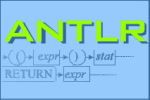
\includegraphics[width=2.5cm]{./planning/img/antlr_logo}
	\vspace{-20pt}
\end{wrapfigure}
\gls{antlr}\footnote{\url{http://www.antlr.org/}}, ANother Tool for Language
Recognition, is a compiler toolkit for creating \glspl{lexer} and \glspl{parser} from grammar
files. It can create these compilers for several different target languages,
including \Gls{java} and \Gls{python}. There exists \gls{antlr} grammar files for the challenges
we are facing: parsing \Gls{c}, \Gls{c} \gls{preprocessor} step and parsing \gls{asnone}. These grammars
configure \gls{antlr} to create \Gls{java} \glspl{lexer} and \glspl{parser} which reads and validates
inputted source code files.

\subsection{PLY}
%---------------
\Gls{aply}\footnote{\url{http://www.dabeaz.com/ply/}} is a \Gls{python} alternative to the
popular \gls{lexer} and \gls{parser} compilers lex and yacc. It also comes with a 95\%
completed \Gls{c} \gls{preprocessor} in case we are required to modify the \gls{preprocessor}
for our \gls{utility}. Other special purpose \glspl{parser} like \gls{pycparser} and
cppheaderparser depends on \Gls{aply}. These are described later in this section.

\subsection{\gls{pycparser}}
%---------------------
\label{sec:pre:pycparser}
There are two \Gls{python} \glspl{library} for parsing \Gls{c} with the same name, but different
capitalization, \gls{pycparser}\footnote{\url{http://code.google.com/p/\gls{pycparser}/}}
and PyCParser\footnote{\url{https://github.com/albertz/PyCParser}}. While they
both aim to solve almost the same problem, the first one appears to have better
documentation, is a more mature project and support more of the \Gls{C99}
specification. \gls{pycparser} requires \Gls{aply} to work.

\subsection{cppheaderparser}
%---------------------------
Cppheaderparser\footnote{\url{http://sourceforge.net/projects/cppheaderparser/}}
is a \gls{parser} for \Gls{c++} \gls{header} files written in \Gls{python}. It is an alternative for
\gls{pycparser} in case we need to parse \Gls{c++} files instead of simple \Gls{c} \gls{header} files.
It also depends on \Gls{aply}.

\subsection{GCC}
%---------------
\label{sec:pre:gcc}
\begin{wrapfigure}{r}{1.5cm}
	\vspace{-20pt}
	
\includegraphics[width=1.5cm]{./planning/img/gcc_logo}
	\vspace{-20pt}
\end{wrapfigure}
GNU Compiler Collection\footnote{\url{http://gcc.gnu.org/}} (\Gls{agcc}) is a
compiler system which has front ends which parse \Gls{c} and \Gls{c++} code, and is written
in \Gls{c} and \Gls{c++}. It can be used in our \gls{utility} as an external tool which does the
parsing and then outputs an intermediate language representation which we can
parse/search to find the \Gls{c} \gls{struct} definitions. Its drawbacks are a lack of
flexibility if we need to change its behaviour, and we will still need to write
a custom \gls{parser} or use something like \gls{GCC-XML} and an \gls{axml} \gls{parser}.

\subsection{\Gls{clang}}
%-----------------
\label{sec:pre:clang}
\begin{wrapfigure}{r}{2.5cm}
	\vspace{-20pt}
	
\includegraphics[width=2.5cm]{./planning/img/llvm_logo}
	\vspace{-20pt}
\end{wrapfigure}
\Gls{clang}\footnote{\url{http://clang.llvm.org/}} is a compiler front end for \Gls{c}, 
\Gls{c++}, \Gls{Objective-C} and \Gls{Objective-C++}, written in \Gls{c++}. \Gls{clang} differ from \Gls{agcc} as it
behaves as a \gls{library} rather than an external tool, but for \Gls{java} we will have to
use it like \Gls{agcc} because there are no \Gls{java}-\Gls{clang} bindings. It supports
outputting the \gls{AST} as \Gls{axml}, which our \gls{utility} then will need to
parse. \Gls{clang} provides bindings for \Gls{python} so there it can be used as a \gls{library},
but its main drawback is, like \Gls{agcc}, a lack of flexibility. \Gls{clang} is a part of
the LLVM toolkit.


%---------------------------------
\section{Configuration Frameworks}
%---------------------------------
\label{sec:pre:config}
This section looks at different configuration frameworks for \Gls{python}. Which we
selected and why is explained in \autoref{sec:pre:configchoice}.

Our \gls{utility} needs a flexible configuration, as some of the information we
shall display does not exist in the files we parse. For example there are no
clear relationship between enumerated values in messages and their names.
These must be provided through a configuration.

\subsection{\gls{asnone}}
%-----------------
\gls{asn1} (\gls{asnone}) for describing data
structures, the standard is defined by \Gls{iso} 8824. \gls{asnone} is used for
representing, encoding, transferring and decoding of data. It provides a
fundamental tool to be used in application, which make it possible to exchange
information in a independent way. There exist two \Gls{python} \glspl{library} for parsing
of  \gls{asnone}, but neither support the 3.x \gls{branch} of \Gls{python}, which we require.

\subsection{\Gls{yaml}}
%----------------
\label{sec:pre:yaml}
\begin{wrapfigure}{r}{3cm}
	\vspace{-30pt}
	
\includegraphics[width=3cm]{./planning/img/pyyaml_logo}
	\vspace{-30pt}
\end{wrapfigure}
\Gls{yaml}\footnote{\url{http://yaml.org/}} (\Gls{yaml} Ain't Markup Language) is a \gls{data serialization} format.
It is designed to be easy to read and write for humans.
\Gls{yaml} syntax was designed to be easily mapped to data types common to most
high-level languages. While most programming languages can use \Gls{yaml} for data
serialization, \Gls{yaml} excels in working with those languages that are
fundamentally built around the three basic primitives. These include the new
wave of agile languages such as \Gls{perl}, \Gls{python}, \GLS{php}, \Gls{Ruby}, and \Gls{Javascript}.

PyYAML\footnote{\url{http://pyyaml.org/}} is a \Gls{yaml} \gls{parser} for the \Gls{python}
programming language, and it is available for both the 2.x and 3.x \gls{branch} of
\Gls{python}. It is licensed under the \Gls{mit} license.

\subsection{configparser}
%------------------------
configparser\footnote{\url{http://docs.python.org/py3k/\gls{library}/configparser.html}}
is a \Gls{python} module to manage user-editable configuration files. The
files are organized into sections, and each section can contain name-value
pairs for configuration data. Value interpolation using \Gls{python} formatting
strings is also supported, to build values that depend on one another.

configparser module is a part of \Gls{python} standard \gls{library}, and therefore does
not require installation or configuration to use.

\subsection{ConfigObj}
%---------------------
ConfigObj\footnote{\url{http://www.voidspace.org.uk/python/configobj.html}} is
a simple but powerful config file reader and writer (originally based on
ConfigParser). Its main feature is that it is very easy to use, with a
straightforward programmer's interface and a simple syntax for config files.
Among others, it has these additional features:
\begin{itemize}
	\item Nested sections (subsections), to any level
	\item List values
	\item Multiple line values
	\item String interpolation (substitution)
	\item Integrated with a powerful validation system
\end{itemize}

\noindent Currently, ConfigObj module exists only for \Gls{python} up to version
2.7. It is under \Gls{bsd} license.


%--------------------------------
\section{Unit Testing Frameworks}
%--------------------------------
\label{sec:pre:testing}
There are many different unit testing frameworks for \Gls{python}. We have evaluated
three of them, to see which best suits our \gls{utility}, which we describe in this
section. In \autoref{sec:pre:testchoice} we describe which we selected and why.

\subsection{py.test}
%-------------------
py.test\footnote{\url{http://pytest.org/latest/}} is a mature, full-featured testing
tool. It runs on \Gls{python} 2.4-3.2, PyPy and Jython-2.5.1 intepreters on both
Windows and Posix platforms. It is well documented and popular in the \Gls{python}
community. The best known project which uses it is PyPy, which has over 16,000
unit tests. py.test discoverers tests automatically by searching for modules,
classes, functions and methods which starts with "test\_". It uses the assert
statement to test variables and values. These implicit behaviours make tests
easier and faster to write, but harder to learn and understand.

\subsection{nose}
%----------------
nose\footnote{\url{http://readthedocs.org/docs/nose/en/latest/}} testing
framework extends \Gls{python}'s unittest \gls{library} to make testing easier.
It provides an alternative test discovery and running process for unittest,
which is intended to mimic the behavior of py.test as much as reasonably
possible without resorting to too much magic. nose support easy-to-write
plugins, and it comes bundled with the most popular ones. It supports both
\Gls{python} 2.x and 3.x \glspl{branch}.

\subsection{Attest}
%------------------
\label{sec:pre:attest}
\begin{wrapfigure}{r}{3.2cm}
	\vspace{-20pt}
	
\includegraphics[width=3.2cm]{./planning/img/pocoo_logo}
	\vspace{-30pt}
\end{wrapfigure}
Attest\footnote{\url{http://packages.python.org/Attest/}} is a test automation
framework for \Gls{python}, emphasising modern idioms and conventions. It supports
test collecting using \Gls{python} decorators, introspection of the assert statement,
treating tests as \Gls{python} modules rather than scripts. Attest is a rather young
framework, with limited features and documentation. Attest is a sub-level
project of the Pocoo project.

\subsection{coverage.py}
%-----------------------
coverage.py\footnote{\url{http://nedbatchelder.com/code/coverage/}} is a tool
for measuring code coverage of \Gls{python} programs. It is typically used to measure
the effectiveness of unit tests, by showing which parts of the code are
exercised by tests. coverage.py support \Gls{python} 2.3 to 3.2. It can output
results in plain text, \Gls{html} and \Gls{axml}.


%---------------------------------
\section{User Documentation Tools}
%---------------------------------
\label{sec:pre:docs}
Some of the non-functional requirements for our \gls{utility} is user documentation.
In this section we describe a tool for writing such documentation, and a free
hosting site for our user documentation.

\subsection{Sphinx}
%------------------
\begin{wrapfigure}{r}{2.7cm}
	\vspace{-20pt}
	
\includegraphics[width=2.7cm]{./planning/img/sphinx_logo}
	\vspace{-20pt}
\end{wrapfigure}
Sphinx\footnote{\url{http://sphinx.pocoo.org/}} is a \Gls{python} tool for writing
documentation, that makes it easy to create intelligent and beautiful
documentation. It is used for the standard \Gls{python} documentation, and it is
popular in the \Gls{python} community. Sphinx uses reStructuredText as its markup
language, which is a easy-to-read, what-you-see-is-what-you-get plain text
markup syntax and \gls{parser} system. Our use case for sphinx is writing
documentation for our \gls{utility}, how to use it and configure it. Sphinx can
generate output in several different formats, including \Gls{html} and latex/pdf.

\subsection{Read the Docs}
%-------------------------
\begin{wrapfigure}{r}{1.2cm}
	\vspace{-20pt}
	
\includegraphics[width=1.2cm]{./planning/img/readthedocs_logo}
	\vspace{-20pt}
\end{wrapfigure}
Read the Docs\footnote{\url{http://readthedocs.org/docs/read-the-docs/}} is a
free hosting of documentation for the open source community. It supports Sphinx
docs written with reStructuredText, and it can automatically pull from Git,
Subversion, Bazaar, and Mercurial repositories. We can configure it so it
automatically pulls and compiles our user documentation from our github
repository whenever we push any changes.


%-------------------------------------------
\section{Integrated Development Environment}
%-------------------------------------------
\label{sec:pre:ide}

\subsection{PyCharm}
%-------------------
\begin{wrapfigure}{r}{3.5cm}
	\vspace{-20pt}
	
\includegraphics[width=3.5cm]{./planning/img/pycharm_logo}
	\vspace{-20pt}
\end{wrapfigure}
PyCharm\footnote{\url{http://www.jetbrains.com/pycharm/}}
is a cross platform, proprietary \Gls{ide} for \Gls{python}. It has good support
for text editing, syntax highlighting, auto indentation, code navigation, code
completion and automatic error checking. There is also a decent debugger and
unit test support that can help finding errors and integrated version control
support (including git), which makes it easy to synchronize with a remote
repository. Most mentioned functions is also paired with keyboard shortcuts.

The downside with PyCharm is that it requires a relative expensive license. It
is, however, possible to apply for classroom licenses that are free of charge.
The latter is a requirement to make this \Gls{ide} a viable option.

\subsection{PyScripter}
%----------------------
\begin{wrapfigure}{r}{3cm}
	\vspace{-20pt}
	
\includegraphics[width=3cm]{./planning/img/pyscripter_logo}
	\vspace{-20pt}
\end{wrapfigure}
PyScripter\footnote{\url{http://code.google.com/p/pyscripter/}}
is a Windows only, open source \Gls{ide} for \Gls{python}. It has support for
basic text editing functions relevant to programming like syntax highlighting,
auto indentation, code completion, debugger and file management. It also has
some support for navigating the code, for example by offering to find the next
point in the code that references a certain variable or function. The mentioned
function mostly has keyboard shortcuts.

It does not have support for automatic error checking in the program, so it
will not alert the user of spelling and syntax errors. It also lacks integration
with any version control systems like git or svn. The code completion and
code navigation is a little lacking. It will for example not suggest importing
files if you reference a class from another module and it cannot give a
complete list of usages of a function.

\subsection{\gls{vim}}
%---------------
\begin{wrapfigure}{r}{1.5cm}
	\vspace{-20pt}
	
\includegraphics[width=1.5cm]{./planning/img/vim_logo}
	\vspace{-20pt}
\end{wrapfigure}
\gls{vim}\footnote{\url{http://www.vim.org/}} is cross-platform, open source text
editor originally created for the Amiga. It is not regarded as an \Gls{ide}, but it
provides all the regular features of text editors, including syntax
highlighting, auto-completion, auto-indentation, searching, multiple undo and
redo. It can be configured to support almost everything modern \Gls{ide}’s support,
and its extensive customizability is considered parts of its strength. But it
is also parts of its weakness, it is very difficult for new \gls{vim} users to learn
how to use it effectively. Therefore we do not suggest any team member which is
not already experienced with \gls{vim} to try it.

\subsection{Summary}
%-------------------
PyCharm is by far the best \Gls{ide} evaluated in terms of functionality, and it is
the one that mirrors \Gls{Eclipse} the most, which is an advantage, since most team
members are best acquainted with \Gls{Eclipse}. It will be the recommended \Gls{ide} for
this project, given that we can acquire classroom licenses.

On the other hand, there is no real reason to dictate the use of \Gls{ide}, since
what determines the productivity of a team member is more how well you know
the specific tool you are using. It will therefore be up to each team member
to choose what \Gls{ide}/text editor they want to use.


%----------------------------------
\section{Evaluation and Conclusion}
%----------------------------------
\label{sec:pre:eval}
In this section we provide a justification for the choices we have made in
regards to process, programming language, and \glspl{library} we will use. Then
in \autoref{sec:pre:framework} we give a brief description of the framework
we will construct for our \gls{utility}.

\subsection{Development Process Choice}
%--------------------------------------
\label{sec:pre:devchoice}
We have chosen \hyperref[sec:pre:scrum]{\Gls{scrum}} for our development strategy.
We do not have a lot of experience with software development either
individually or as a team, so we have little personal knowledge of how much
we are able to produce, and the task may present challenges that we are not
prepared for when the project starts. For these reasons we believe that we
need to take an agile approach to this project. This way, we may both learn as
we go, and adjust later iterations by the result of the previous. We may also
have something to deliver even if we do not have time to implement all the
desired features.

The \Gls{scrum} methodology fits these goals perfectly, and is therefore a natural
choice. The risk factor here is that all team members are mostly unfamiliar
with \Gls{scrum}, while we have at least a little knowledge of waterfall. We do,
however, think that the time and risk of learning will not outweigh
the benefit it will give us over waterfall.

\subsection{Programming Language Choice}
%---------------------------------------
\label{sec:pre:langchoice}
We originally selected \hyperref[sec:pre:java]{\Gls{java}} as our programming
language because it would run on all the platforms required, it offered
automatic memory management so it would be easier to debug, and it was the only
language everyone on the team had experience with.

We looked at \hyperref[sec:pre:antlr]{\gls{antlr}} for generating a
\Gls{c} \gls{lexer} and \gls{parser} in \Gls{java}, which looked very promising. It also provided
grammar files for creating a \Gls{c} \gls{preprocessor} in \Gls{java}. Closer evaluation revealed
that the \Gls{c} \gls{preprocessor} grammar was written in 2006, and had stopped working in
2008 as newer versions of \gls{antlr} was not backwards compatible. Also the
generated \Gls{c} \gls{parser} only validated \Gls{c} code, it did not create an \gls{AST} which we could traverse.
This meant that using \Gls{java} and \gls{antlr} would
require us to modify these grammars to suite our needs, and \gls{antlr}'s lack of
documentation became a significant risk for our project.

These issues and feedback from our customer made us evaluate \Gls{python} for
developing our \gls{utility}. We found several \glspl{library} for parsing \Gls{c} files, and
even one for parsing \Gls{c++} \gls{header} files. These are described in
\autoref{sec:pre:parser}.

We decided to use \hyperref[sec:pre:python]{\Gls{python}} for this project because
the parsing \glspl{library} for \Gls{python} came in working condition with decent
documentation, and because we were able to create a small working prototype
in \Gls{python} in just a few hours. We estimate that it would take at least a week
to achieve the same result in \Gls{java}.

A challenge with our decision is the fact that not all team members have
sufficient experience with \Gls{python}. Most team members must therefore do some
self study before we start the first sprint.

\subsection{Parsers Libraries \& Tools Choice}
%---------------------------------------------
\label{sec:pre:parserchoice}
We outlined three different approaches for parsing \Gls{c} \gls{header} files. The first approach is to
write a custom \gls{parser} ourself, the second is to use a \Gls{c} parsing \gls{library}, and the
third is to use a toolkit \gls{parser} like \hyperref[sec:pre:gcc]{\Gls{agcc}} and
\hyperref[sec:pre:clang]{\Gls{clang}}.

We felt that writing our own \Gls{c} \gls{parser} with \Gls{c} \gls{preprocessor} would possibly take
up a lot, if not all, of the available project time. The third option would add
a large dependency which our customer want to avoid if possible. \Gls{agcc} and \Gls{clang}
can be challenging to install and use on Windows.

Therefore using a \Gls{c} \gls{parser} \gls{library} would be the best solution, and as mentioned
above, \Gls{java} with \gls{antlr} proved challenging. So we evaluated \Gls{python} \gls{parser}
\glspl{library}.

We decided to use \hyperref[sec:pre:pycparser]{\gls{pycparser}}. We favored \gls{pycparser}
over PyCParser and cppheaderparser because it has better documentation, it
seemed to be a more mature project, and it supports the most of the \Gls{C99}
specification. \gls{pycparser} depends on \Gls{aply}, so our \gls{utility} will also depend on it.

For \Gls{c} \gls{preprocessor} we have selected to use a tool for Windows which comes with
\gls{pycparser}, on Mac we will use the one which comes with XCode, and on other
platforms we will either use \Gls{agcc} or tools which comes with the platform. If we
need to modify a \Gls{c} \gls{preprocessor} we might use \Gls{aply}'s incomplete \Gls{c} \gls{preprocessor}.

\subsection{Configuration Framework Choice}
%------------------------------------------
\label{sec:pre:configchoice}
We have listed a summary of some of the advantages and drawbacks of the
different configuration frameworks we looked at in \autoref{tab:pre:config}.
\begin{table}[htbp] \footnotesize \center
\caption{Configuration summary\label{tab:pre:config}}
\noindent\makebox[\textwidth]{%
\begin{tabularx}{1.1\textwidth}{X X X X X}
	\toprule
	& \Gls{yaml} & configparser & ConfigObj & \gls{asnone} \\
	\midrule
	Advantages &
	+Simplicity\newline +Flexibility &
	+Easy to use &
	+Easy to use\newline +Flexibility\newline +Nesting\newline +Type \newline\hspace*{3mm}validation &
	+Customer \hspace*{3mm}wants it \\
	\addlinespace
	Drawbacks &
	-External \gls{library}\newline -No type \newline\hspace*{2mm}validation &
	-Lacks nesting\newline -Lacks lists\newline -No type \newline\hspace*{2mm}validation &
	-External \gls{library}\newline -Lacks lists &
	-External \gls{library}\newline -Too generic \\
	\addlinespace
	Latest version & 3.10 & 3.2 & 4.7.2 & 0.0.13 \\
	\Gls{python} \gls{branch} & 2.7 and 3.3 & 2.7 and 3.3 & 2.7 & 2.7 \\
	License & \Gls{mit} & PSF L & \Gls{bsd}-new & \Gls{bsd} \\
	\bottomrule
\end{tabularx}}
\end{table}

We decided to use \hyperref[sec:pre:yaml]{YAML} for handling configuration
files, as it covered most of our requirements. Because we decided to use the
latest version of \Gls{python}, version 3.2.2, the range of possible configuration
frameworks was reduced. Therefore, although \gls{asnone} and ConfigObj are very
suitable for our task, they were eliminated (those \glspl{parser} are available
only up to version 2.7), which left us 2 main possibilities: \Gls{yaml} and
configparser. configparser turned out to be insufficient for us, mainly because
it lacked lists. These we need for description of hierarchical structures of
the \Gls{c} \glspl{header}. \Gls{yaml} has only two minor disadvantages we should be aware of.
First, there is no type validation mechanism, so we will have to create our
validation manually. Second, it is an external \gls{library}. We find this drawback
minor for now but it can turn out to be a problem in the future. Except for
these issues, \Gls{yaml}, more specifically pyYAML, seems to have a good potential
for creating flexible configuration support for our \gls{utility}.

\subsection{Unit Testing Framework Choice}
%-----------------------------------------
\label{sec:pre:testchoice}
The three frameworks we looked at  are very similar, being modern \Gls{python}
testing frameworks. They differ in maturity and what is often called magic in
the \Gls{python} community.

py.test is the most mature but also the most magic, it uses a lot of
introspection to discover tests and it has no \Gls{api}. nose is heavily influenced
by py.test, but it tries to be more explicit, and provides an \Gls{api}. Attest is
the youngest testing framework, and like nose, has less magic and focuses on
providing a very pythonic \Gls{api}. Being the youngest also means it has the least
documentation, functionality and plugins. Therefore Attest might be the easiest
testing framework to learn. Therefor we decided to use
\hyperref[sec:pre:attest]{Attest} for unit testing of our \gls{utility}.

\subsection{Our Framework}
%-------------------------
\label{sec:pre:framework}
Our \gls{utility} will need to take as input \Gls{c} \gls{header} files, search through them to
find \gls{struct} definitions, and create \Gls{lua} scripts which dissects the \glspl{struct} in
\hyperref[sec:pre:wireshark]{Wireshark}.

To find the \glspl{struct} we will use \gls{pycparser} to parse the input files, create an
\gls{AST}, and to find the \gls{struct} definitions. We will use pyYAML to
read configuration from file, which together with the \gls{struct} definitions will
be placed in some suitable data structures for generating \glspl{dissector}.

The versions of the different tools and \glspl{library} we are using can be found in
\autoref{tab:pre:versions}.
\begin{table}[!h] \footnotesize \center
\vspace{-10pt}
\caption{Versions of tools and \glspl{library}\label{tab:pre:versions}}
\begin{tabular}{l l l}
	\toprule
	Library/Tool & Version & Why \\
	\midrule
	\Gls{python} & CPython 3.2.2 & Latest stable standard \Gls{python} implementation \\
	\gls{pycparser} & 2.05-dev & Development version, for \_Bool support \\
	pyYAML & 3.10 & Latest stable version \\
	\Gls{aply} & 3.4 & Latest stable version \\
	Attest & 0.6-dev & Development version, for \Gls{python} 3.2 support \\
	Sphinx & 1.0.8 & Latest stable version \\
	WireShark & 1.7.0-SVN & Latest nightly build, for \Gls{lua} support \\
	\bottomrule
\end{tabular}
\vspace{-10pt}
\end{table}


%-----------------------------
\section{IP Rights \& License}
%-----------------------------
\label{sec:pre:license}
The customer has explained that they do not intend to distribute our \gls{utility},
and that we are free to license it as open source if we want to, under
whichever license we feel is most suited. They suggested GNU\footnote{\url{http://www.gnu.org/}} \Gls{gpl} as \Gls{wireshark}
is released under it.

We needed to consider the licenses of the \glspl{library} and tools we depend upon
when we decided which license to use. This is summarized by
\autoref{tab:pre:licenses}.
\begin{table}[!h] \footnotesize \center
\vspace{-20pt}
\caption{Licenses\label{tab:pre:licenses}}
\begin{tabular}{l l}
	\toprule
	\Gls{wireshark} & GNU \Gls{gpl} \\
	\Gls{aply} & \Gls{bsd}-new \\
	\gls{pycparser} & \Gls{bsd}-new \\
	pyYAML & \Gls{mit} \\
	\midrule
	Our \gls{utility} & \Gls{bsd}-new \\
	\bottomrule
\end{tabular}
\vspace{-10pt}
\end{table}

\noindent Some of the requirements for our \gls{utility} might require us to modify
the \Gls{c} \gls{preprocessor} in \Gls{aply} and the \gls{pycparser} \gls{library}, which made us consider
the new 2-clause \Gls{bsd} license the most suited for us. Since it also gives us the
option to later move to a more restrictive license like \Gls{gpl}, we decided to use
it.
